% Copyright (c) 2008-2009 solvethis
% Copyright (c) 2010-2017,2021 Casper Ti. Vector
% Copyright (c) 2021 Kurapica
% Copyright (c) 2021 iofu728
% Copyright (c) 2025 CS_icez
% All rights reserved.
%
% Redistribution and use in source and binary forms, with or without
% modification, are permitted provided that the following conditions are
% met:
%
% * Redistributions of source code must retain the above copyright notice,
%   this list of conditions and the following disclaimer.
% * Redistributions in binary form must reproduce the above copyright
%   notice, this list of conditions and the following disclaimer in the
%   documentation and/or other materials provided with the distribution.
% * Neither the name of Peking University nor the names of its contributors
%   may be used to endorse or promote products derived from this software
%   without specific prior written permission.
%
% THIS SOFTWARE IS PROVIDED BY THE COPYRIGHT HOLDERS AND CONTRIBUTORS "AS
% IS" AND ANY EXPRESS OR IMPLIED WARRANTIES, INCLUDING, BUT NOT LIMITED TO,
% THE IMPLIED WARRANTIES OF MERCHANTABILITY AND FITNESS FOR A PARTICULAR
% PURPOSE ARE DISCLAIMED. IN NO EVENT SHALL THE COPYRIGHT HOLDER OR
% CONTRIBUTORS BE LIABLE FOR ANY DIRECT, INDIRECT, INCIDENTAL, SPECIAL,
% EXEMPLARY, OR CONSEQUENTIAL DAMAGES (INCLUDING, BUT NOT LIMITED TO,
% PROCUREMENT OF SUBSTITUTE GOODS OR SERVICES; LOSS OF USE, DATA, OR
% PROFITS; OR BUSINESS INTERRUPTION) HOWEVER CAUSED AND ON ANY THEORY OF
% LIABILITY, WHETHER IN CONTRACT, STRICT LIABILITY, OR TORT (INCLUDING
% NEGLIGENCE OR OTHERWISE) ARISING IN ANY WAY OUT OF THE USE OF THIS
% SOFTWARE, EVEN IF ADVISED OF THE POSSIBILITY OF SUCH DAMAGE.

% CS_icez: I modified this file while referencing https://github.com/CasperVector/pkuthss/blob/master/doc/example/chap/origin.tex
{
    \ctexset{
        chapter = {
            afterskip = {8bp}
        },
        subsection = {
            format+ = {\centering}, beforeskip = {0bp}, afterskip = {20bp}
        }
    }
    \centeredchapterformat
    \specialchap{北京大学学位论文原创性声明和使用授权说明}

    % 学校书面要求本页面不要页码,但在给出的 Word 模版中又有页码。
    % 此处以学校书面要求为准。
    \thispagestyle{empty}
	
    % 替换扫描pdf,去除includegraphics前注释
    % \begin{textblock}{1}(-0.8,-0.08)
    %   \colorbox{white}{
    %       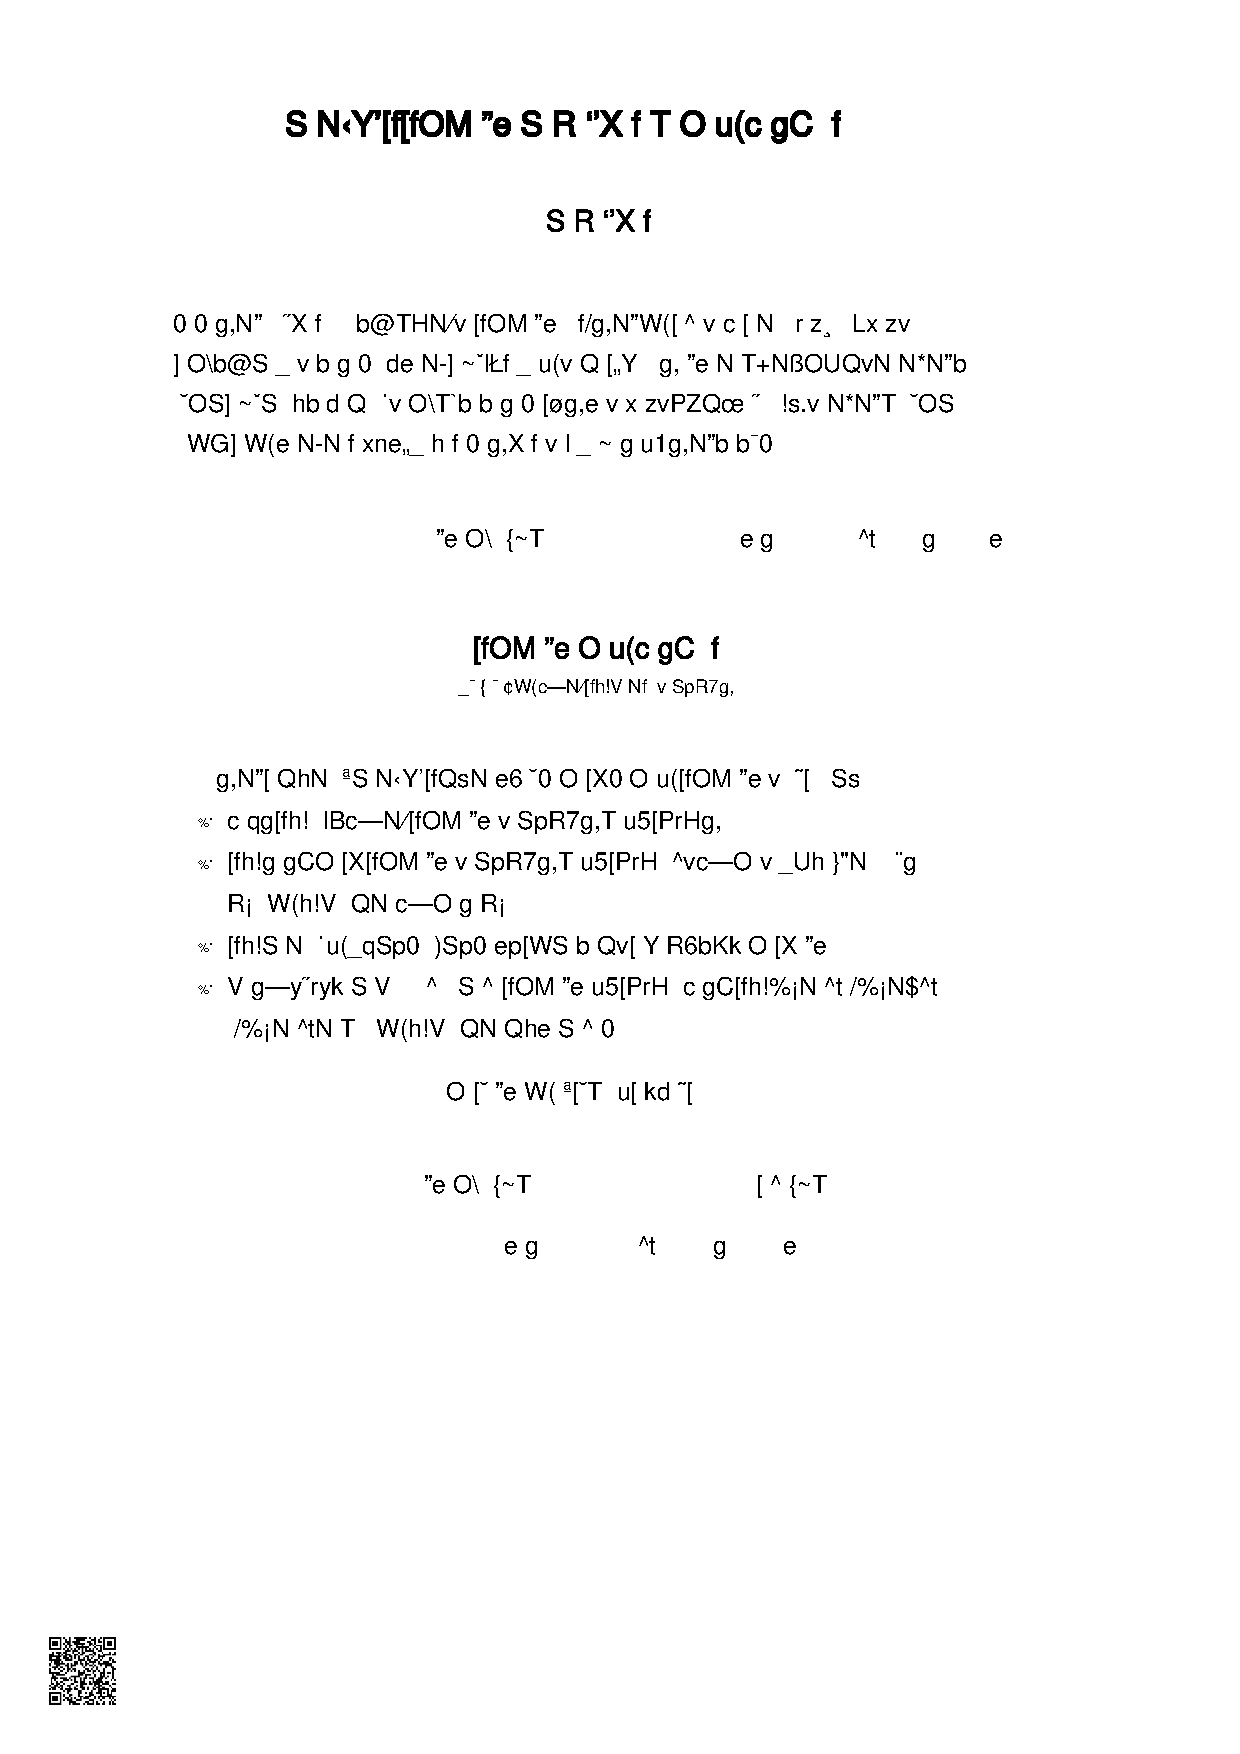
\includegraphics[height = 1.2448\textheight]{img/lwsm_180xxxxxxx.pdf}
    %   }
    % \end{textblock}

    \subsection*{\textbf{原创性声明}}
    
    本人郑重声明:
    所呈交的学位论文,是本人在导师的指导下,独立进行研究工作所取得的成果。
    除文中已经注明引用的内容外,
    本论文不含任何其他个人或集体已经发表或撰写过的作品或成果。
    对本文的研究做出重要贡献的个人和集体,均已在文中以明确方式标明。
    本声明的法律结果由本人承担。
    \vskip 2em
    \rightline{论文作者签名:\hspace{9em}}
    \rightline{日期:\hspace{2em}年\hspace{2em}月\hspace{2em}日}

    \vspace{100bp}
    \subsection*{\textbf{学位论文使用授权说明}}
    
    本人完全了解北京大学关于收集、保存、使用学位论文的规定,即:
    \begin{itemize}
        \item 按照学校要求提交学位论文的印刷本和电子版本;
        \item 学校有权保存学位论文的印刷本和电子版,
            并提供目录检索与阅览服务,在校园网上提供服务;
        \item 学校可以采用影印、缩印、数字化或其它复制手段保存论文;
    \end{itemize}
    \vskip 3em
    \rightline{论文作者签名:\hspace{6.5em}导师签名:\hspace{3.5em}}
    \rightline{日期:\hspace{2em}年\hspace{2em}月\hspace{2em}日\hspace{5em}}
}

\defaultchapterformat

% vim:ts=4:sw=4